\chapter{リアルタイム看板認識APIの実装}
\label{chapter:implement_recog}
本章では,リアルタイムで看板認識を行うために実装したAPIについて述べる.

\section{システムの概要}
  カメラを通して見た映像に店舗情報を付与するために,街を撮影した画像から看板を認識し,その結果を返却するAPIを実装した\cite{Kitamura:2018}.
  システムは(1)看板領域の検出,(2)看板の分類,の2段階の処理を行うことで看板を認識し,画像内の看板の座標及び店舗をJSON形式で返却する.
  まず,システムはYOLOv2 \cite{Redmon:2017}を用いて画像の中から看板を囲む長方形の枠線であるバウンディングボックスを検出する.
  次に,YOLOv2によって切り出された看板をVGG16 \cite{Simonyan:2015}を用いて店舗毎にクラス分けを行う.
  これにより,少ない教師データから高精度での看板認識が可能になる.
  リアルタイムで画像認識を行うためには,ハイスペックなGPUを搭載したマシンが必要であるため,スマートフォン等のモバイルデバイスでこれを行うことは困難である.
  そのため,GPUを搭載したマシン上にWeb APIサーバを構築し,モバイルデバイスから一定ミリ秒毎にこのAPIを呼び出すことによって,リアルタイムでの看板認識を実現する.
  
\section{対象とするデータ}
\label{section:target_data}
  本稿では,大阪府高槻市のJR高槻駅と阪急高槻市駅の間に位置する商店街の一区域を対象としたプロトタイプを実装する.
  プロトタイプでは,図\ref{figure:recog_map}の赤線部で示されている高槻本通の$100\, \mathrm{m}$区間において,オープンソースの地理情報システムであるOpenStreetMap(以下,OSMと記す)\cite{Haklay:2008}に2018年10月1日時点でデータが存在した(1)赤から 高槻店,(2)メサベルテ 高槻店,(3)高槻ちゃぶちゃぶ,(4)炭焼酒場 森田屋 高槻店,(5)全席個室居酒屋 北海の恩返し 高槻店,(6)肉丼専門店 高槻肉劇場,(7)磯丸水産 高槻店,(8)おだいどこはなれ 高槻店,(9)ぢどり亭 高槻店,(10)ビリヤード・ダーツ \& Food Bar OzBuddy,(11)小だるま JR高槻駅前店,(12)焼肉・しゃぶしゃぶ食べ放題 ぷくぷく 高槻店,(13)甲南チケット 高槻本通店,(14)セブン--イレブン 高槻高槻町店,(15)駿河屋,の15店舗を対象とする.
  \begin{figure}[tb]
    \centerline{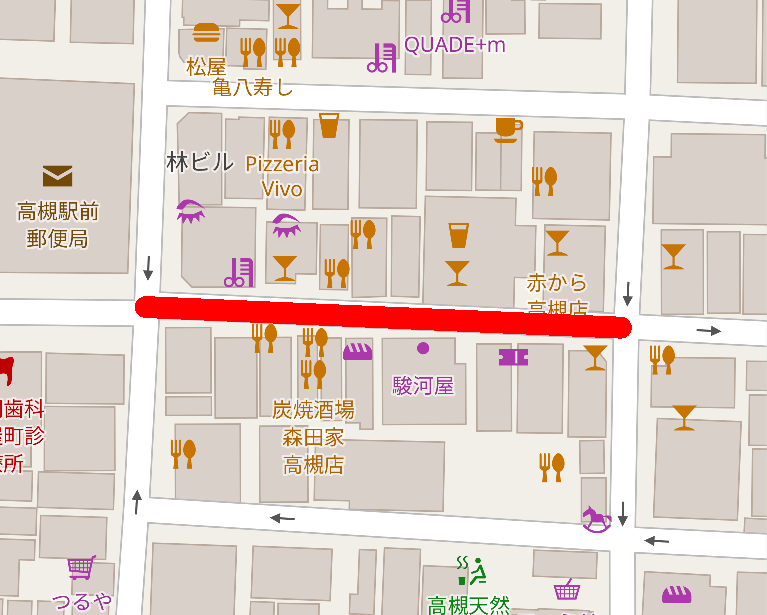
\includegraphics[width=\columnwidth, clip]{recog_map.pdf}}
    \caption{対象とする区域}
    \label{figure:recog_map}
  \end{figure}

\section{看板領域の抽出}
  YOLOv2は9,000種類を超えるオブジェクトの領域推定と分類が可能であるため,YOLOv2のみを用いても看板領域の検出及び分類は可能である.
  しかし,将来的に様々な商店街に対応させるためには,対象とする全ての店舗の看板画像を学習させ1つのモデルを生成する必要があるため,汎用性に欠けるという問題がある.
  そのため,学習させるオブジェクトのクラスは``signboard''の1クラスとし,YOLOv2は看板領域の検出のみに用いる.
  \subsection{アノテーション}
    看板領域をアノテーションするために,画像内に存在するオブジェクトのバウンディングボックスを容易にラベリングできるツールであるBBox-Label-Tool\footnote{\url{https://github.com/puzzledqs/BBox-Label-Tool}(2019/1/26存在確認)}とPython\footnote{\url{https://www.python.org}(2019/1/26存在確認)} 2.7.14を用いる.
    学習に用いる画像は,対象とする地域において複数の店舗が写るよう様々な角度から撮影した650枚の写真を用いる.
    各画像について,対象とする店舗の看板の左上と右下の座標,クラス``signboard''をそれぞれ人手でアノテーションした.
    アノテーションの例を図\ref{figure:annotation}に示す.
    \begin{figure}[tb]
      \centerline{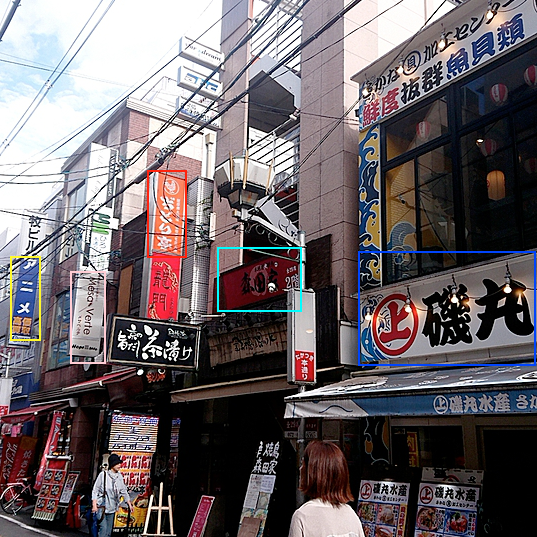
\includegraphics[width=\columnwidth, clip]{annotation.png}}
      \caption{アノテーションの例}
      \label{figure:annotation}
    \end{figure}
    その後,アノテーションしたデータをYOLOv2で用いられているフォーマットに,Python 3.7.0とスクリプト\footnote{\url{https://github.com/Guanghan/darknet/blob/master/scripts/convert.py}(2018/1/27存在確認)}を用いて変換する.
    これらのデータをトレーニングセットとして585枚,テストセットとして65枚に無作為に分類した.
  \subsection{学習}
    YOLOv2では,入力画像を$S \times S$のグリッドに区切り,グリッド毎に,ある一定のアスペクト比を持つ$B$個の矩形領域の中心座標$(x, y)$,そして矩形内に物体が存在する確率を予測する.
    さらに,各矩形に何らかの物体が存在するとき,その物体がどのクラスに属するかを示す事後確率も予測する.矩形領域,物体の存在確率,クラスの事後確率の予測を,YOLOv2では一つの損失関数に統合している.
    矩形領域の中心座標と大きさに関する損失関数を$Loss_{box}$,存在確率に関するものを$Loss_{conf}$,クラスの事後確率のものを$Loss_{p}$としたとき,統合した損失関数を次式に示す.
    \begin{equation}
      Loss = Loss_{box} + Loss_{conf} + Loss_{p}
    \end{equation}

    また,それぞれの損失関数は次式で定義される.
    \begin{align}
      Loss_{box} = &\lambda_{coord} \sum_{i}^{S^2} \sum_{j}^{B} \mathbbm{1}_{ij}^{obj} (x_{ij}^{pred} - x_{ij}^{truth})^2 \\
      &+ (y_{ij}^{pred} - y_{ij}^{truth})^2 + (w_{ij}^{pred} - w_{ij}^{truth})^2 + (h_{ij}^{pred} - h_{ij}^{truth})^2 \notag \\
      Loss_{conf} = &\lambda_{conf}^{obj} \sum_{i}^{S^2} \sum_{j}^{B} \mathbbm{1}_{ij}^{obj}
      \{ conf_{ij}^{pred} - iou(box_{ij}^{pred}, box_{ij}^{truth}) \}^2 \\
      &+ \lambda_{conf}^{no\_obj} \sum_{i}^{S^2} \sum_{j}^{B} \mathbbm{1}_{ij}^{no\_obj} (conf_{ij}^{pred})^2 \notag \\
      Loss_{p} = &\lambda_{prob} \sum_{i}^{S^2} \sum_{j}^{B} \mathbbm{1}_{ij}^{obj}
      \{ p_{ij}^{pred} (c) - p_{ij}^{truth} (c) \}^2
    \end{align}

    ここで,添字$pred$,$truth$が付与された変数がそれぞれ予測値,正解を示す.また,$\mathbbm{1}_{i}^{obj}$は,何らかの物体がセル$i$に存在するかどうかを示し,存在すれば1,存在しなければ0である.$\mathbbm{1}_{ij}^{obj}$は,セル$i$内の$j$番目の矩形候補が,その物体の予測の「担当」であることを示す.
    $\mathbbm{1}_{i}^{no\_obj}$は,セル$i$に物体が存在すれば0,存在しなければ1である.
    また,$iou(A, B)$は,矩形$A$と$B$のIntersection over Union(IoU)を表し,$p(c)$はセル$i$内の$j$番目の矩形候補内に物体が存在するとき,それがクラス$c$である事後確率を表す.また,$\lambda_{coord} = 1.0$,$\lambda_{conf}^{obj} = 5.0$,$\lambda_{conf}^{no\_obj} = 1.0$(ただし,$iou$が閾値未満のとき),$\lambda_{prob} = 1.0$である\cite{Nishikawa:2018}.

    上記の学習データを,1クラスのR-CNNとしてYOLOv2で学習させる.
    学習データは$416 \times 416$の正方形にリサイズし,パラメータとしてバッチサイズは64,分割数は8,学習率は$10^{-3}$,慣性は0.9,荷重減衰は0.0005を与え反復回数は1,000回とする.
    少ない学習データからモデルを作成するため,22層の畳み込み層と5層のプーリング層からなる学習済みモデルであるDarknet19モデル\footnote{\url{https://pjreddie.com/darknet}(2019/1/27存在確認)}を用いる.
    Darknet19モデルの最後の畳み込み層を取り除き,フィルタの数が1024である3層の$3 \times 3$の畳み込み層と,フィルタサイズが30である1層の$1 \times 1$の畳み込み層を加え,学習を行う.
    学習に用いたマシンのスペック表\ref{table:machine}に示す.

    \begin{table}[tb]
      \caption{看板画像の学習と検出に用いたマシンのスペック}
      \label{table:machine}
      \begin{center}
        \begin{tabular}{c|c}
          \hline\hline
          \textbf{要素} & \textbf{スペック} \\
          \hline
          CPU & Intel (R) Core (TM) i7-8700K @ 3.70 GHz \\
          RAM & 16 GB \\
          GPU & NVIDIA GeForce GTX 1080 \\
          VRAM & 12 GB \\
          OS & Ubuntu 17.10 \\
          \hline
        \end{tabular}
      \end{center}
    \end{table}

  \subsection{評価}
    看板領域抽出の精度を評価するために,領域の一致具合を評価する手法であるIoUを用いる.
    正しい看板の領域を$GT$,看板と推定された領域を$PR$とすると,IoU値は,
    \begin{equation}
      IoU = \frac{GT \cap PR}{GT \cup PR}
    \end{equation}
    と定義される.
    1,000回の反復学習の時点において,average lossは0.526,8分割されているIoU値の平均は0.850であった.
    損失のグラフを図\ref{figure:yolo_loss}に示す.

    \begin{figure}[tb]
      \centerline{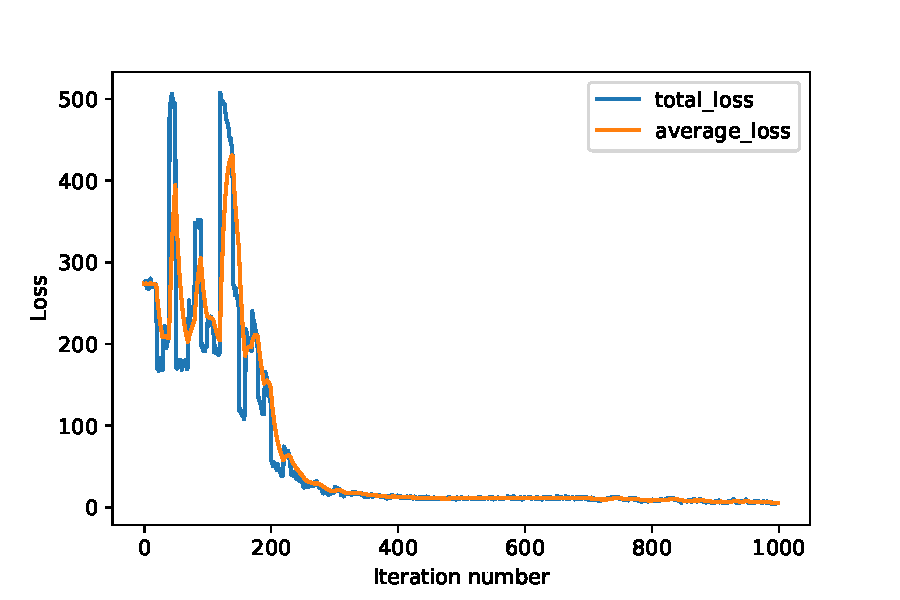
\includegraphics[width=\columnwidth, clip]{yolo_loss.pdf}}
      \caption{YOLOv2による学習誤差曲線}
      \label{figure:yolo_loss}
    \end{figure}

\section{抽出した看板の分類}
  YOLOv2で抽出した看板領域を分類するために,VGG16を用いる.
  VGG16とは,画像データベースのImageNet\footnote{\url{http://www.image-net.org}(2019/1/29存在確認)}に登録されている120万枚の画像を1,000カテゴリに分類したCNNのモデルである.
  VGG16は13層の畳み込み層と3層の全結合層の計16層からなるモデルであり,この全結合層を取り除き,新たに全結合層を追加する転移学習を用いることによって,少ないデータから短時間で高精度のモデルを構築できる.
  本稿では,ニューラルネットワークのライブラリであるKeras\cite{Chollet:2015}で実装されたVGG16を用いて学習を行う.

  \subsection{学習データ}
    学習に用いるデータは,\ref{section:target_data}節で述べた15店舗の看板を,YOLOv2に用いたものとは別に各店舗100枚ずつ様々な角度から撮影した写真を計1,500枚容易し,人手で看板部分のみを切り出した.
    切り出した写真を,1店舗につきトレーニングセットとして50枚,バリデーションセットとして25枚,テストセットとして25枚に無作為に分類した.
    
  \subsection{学習}
    上記の学習データを,サイズは$224 \times 224$,バッチサイズは16,学習率は$10^{-4}$,慣性は0.9,エポック数は50として,表\ref{table:machine}のマシンを用いて学習させる.
    1エポックにつき24回反復して学習を行う.
    学習データが少ないため,トレーニングセットをKerasのImageDataGenerator\footnote{\url{https://keras.io/preprocessing/image}(2019/1/29存在確認)}クラスを用いてせん断変換したり,拡大縮小したり,水平方向に反転したりすることによって十分な量となるまで拡張しながら学習を行う.
    損失関数には,次式で示す15クラスの交差エントロピーを用いる.
    \begin{equation}
      E = -\frac{1}{N} \sum_{n=1}^{N} \sum_{k=1}^{15} t_{nk} \log y_{nk}
    \end{equation}
    ここで,$N$はデータ数,$y_k$はニューラルネットワークの出力,$t_k$は正解ラベルを表す.

  \subsection{評価}
    学習過程におけるトレーニングデータとバリデーションデータの精度と損失のグラフを図\ref{figure:vgg_training}に示す.
    50エポック時点でのトレーニングデータの精度は0.987,損失は0.097,バリデーションデータの精度は0.963,損失は0.156であった.
    評価指標に関しては,真に正であり,かつ予測結果も正であるデータ数をTrue Positive(TP),真に正であるが,予測結果が負であるデータ数をFalse Negative(FN),真に負であるが,予測結果が正であるデータ数をFalse Positive(FP),真に負であり,かつ予測結果も負であるデータ数をTrue Negative(TN)とすると,正と予測した場合の中で実際にそれが正しい割合である適合率(Precision),再現率実際に正である場合の中で正であると予測されたものの割合である再現率(Recall),適合率と再現率の調和平均であるF値は次式で定義される\cite{Richert:2013}.

    \begin{align}
      Precision = &\frac{TP}{TP+FP} \\
      Recall = &\frac{TP}{TP+FN} \\
      F = &\frac{2 Recall \cdot Precision}{Recall + Precision}
    \end{align}
    
    テストデータを用いて各クラス毎に上記の評価指標を計算した結果を表\ref{table:recog_result}に示す.
    各評価指標について,全クラスの結果の平均であるマクロ平均を算出した.
    その結果,適合率は0.960,再現率は0.955,F値は0.956であり,このモデルは看板画像のクラスを分類するために十分な精度があるといえる.

    \begin{figure}[tb]
      \centerline{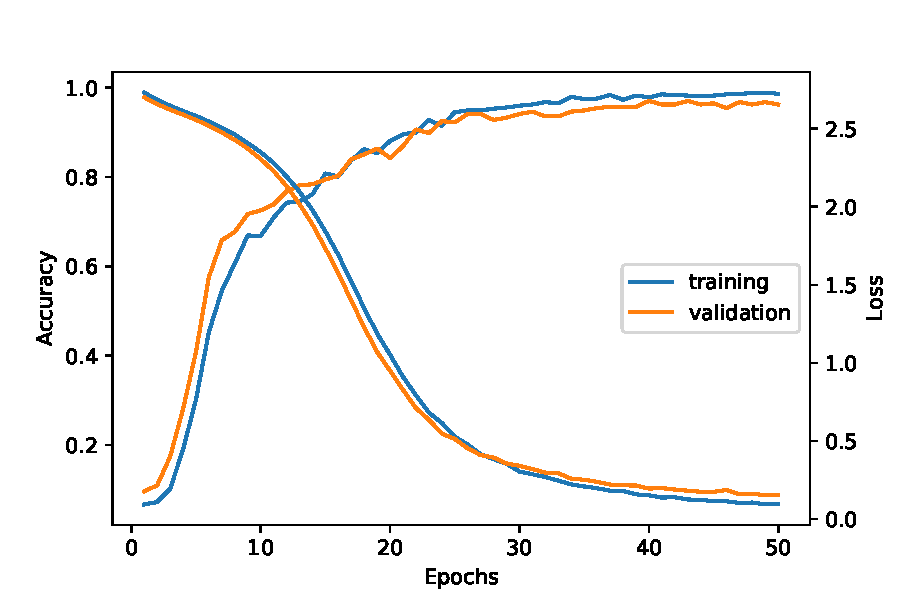
\includegraphics[width=\columnwidth, clip]{vgg_training.pdf}}
      \caption{VGG16による学習誤差曲線}
      \label{figure:vgg_training}
    \end{figure}

\section{APIの実装}
  モバイルデバイスでリアルタイムに看板を認識するために,画像を送信すると,画像内の看板領域と,そのクラスを返却するAPIを実装する.
  APIは,Python 3.6.5とWeb APIフレームワークであるFalcon \footnote{\url{https://falconframework.org}(2019/2/4存在確認)}を用いて構築した.
  サーバには,表\ref{table:machine}に示す,学習に用いたものと同一のマシンを用いる.
  まず,クライアントがAPIに画像をPOSTリクエストとして送信すると,サーバはTensorflow 1.0\cite{Abadi:2016}で実装されたYOLOv2により画像内の看板領域が検出され,切り出される.
  次に,切り出された看板画像をVGG16によってクラス分けを行い,どの店舗の看板なのかを識別する.
  最後に,画像内に存在する全て看板領域の左上と右下の座標,店舗のクラスを格納したJSONデータを生成し,クライアントに返却する.
  このAPIを500ミリ秒毎に呼び出すことによって,モバイルデバイスでのリアルタイムな看板認識が可能になる.

\section{フィールド実験}
  構築したモデルを用いて,実環境でも店舗を識別できるか確認するために,スマートフォンのカメラで撮影した画像をAPIに送信し,結果を表示するAndroidアプリケーションをKotlin\footnote{\url{https://kotlinlang.org}(2019/1/29存在確認)}を用いて実装した.
  実装したアプリケーションを用いて,各店舗の前で写真を撮影し,10回ずつAPIに画像を送信するフィールド実験を行なった.
  実験では,(a)看板領域が正しく検出された回数,(b)看板領域が正しく検出された場合の内,看板画像が正しくクラス分けされた回数,をそれぞれ測定した.
  実験結果を表\ref{table:recog_result}に示す.
  看板領域検出の再現率は0.947,看板領域が正しく検出された場合の内,看板画像のクラス分けの再現率は0.944であり,全体の再現率は0.893であった.
  500ms毎にAPIを呼び出すことによって,リアルタイムでの認識も可能であった.
  考察として,図\ref{figure:recog_discussion}に示す「おだいどこはなれ」のように,同一の店舗が類似していない複数の看板を掲示している場合,本稿では1つの看板のみを学習させていたため,テストデータの精度は高かったものの,実世界での認識の精度は低くなる傾向が見られた.

  \begin{table}[t]
    \caption{モデルの評価及びフィールド実験の結果}
    \label{table:recog_result}
    \begin{center}
      \begin{tabular}{cc|ccc|cc}
        \hline\hline
        \textbf{店舗} & \textbf{看板画像} & \textbf{適合率} & \textbf{再現率} & \textbf{F値} & \textbf{(a)} & \textbf{(b)} \\ \hline
        (1) & 
        \begin{minipage}{40mm}
          \centering
          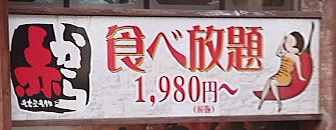
\includegraphics[clip, height=2zh]{akakara.png}
        \end{minipage} & 
        1.000 & 1.000 & 1.000 & % akakara
        9 & 9 \\
        (2) & 
        \begin{minipage}{40mm}
          \centering
          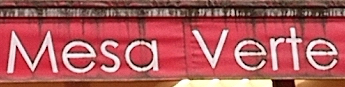
\includegraphics[clip, height=2zh]{mesaverte.png}
        \end{minipage} &
        0.962 & 1.000 & 0.980 & % mesaverte
        10 & 10 \\
        (3) & 
        \begin{minipage}{40mm}
          \centering
          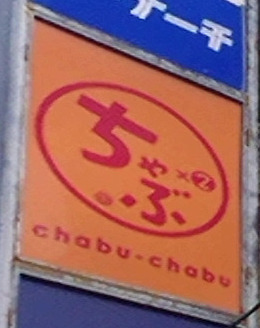
\includegraphics[clip, height=2zh]{chabuchabu.png}
        \end{minipage} &
        1.000 & 1.000 & 1.000 & % chabuchabu
        9 & 9 \\
        (4) & 
        \begin{minipage}{40mm}
          \centering
          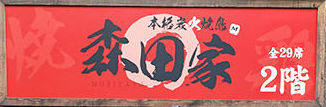
\includegraphics[clip, height=2zh]{moritaya.png}
        \end{minipage} & 
        0.767 & 0.920 & 0.836 & % moritaya
        10 & 10 \\
        (5) & 
        \begin{minipage}{40mm}
          \centering
          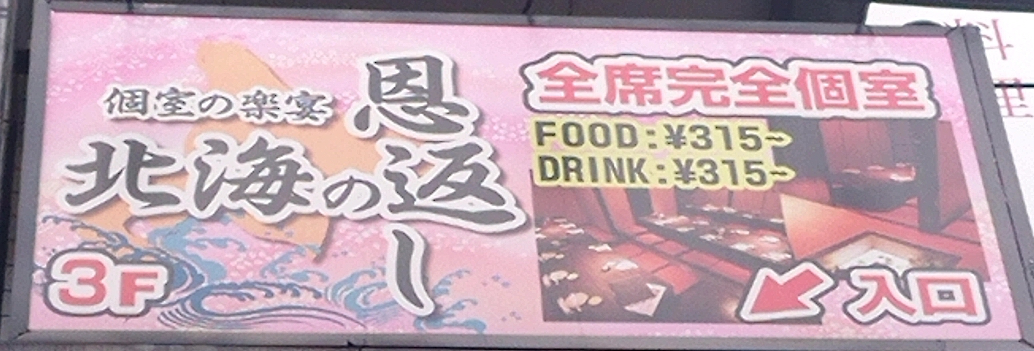
\includegraphics[clip, height=2zh]{hokkai.png}
        \end{minipage} & 
        0.962 & 1.000 & 0.980 & % hokkai
        10 & 10 \\
        (6) & 
        \begin{minipage}{40mm}
          \centering
          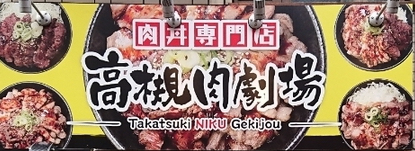
\includegraphics[clip, height=2zh]{nikugekijo.png}
        \end{minipage} &
        0.800 & 0.960 & 0.873 & % nikugekijo
        9 & 9 \\
        (7) & 
        \begin{minipage}{40mm}
          \centering
          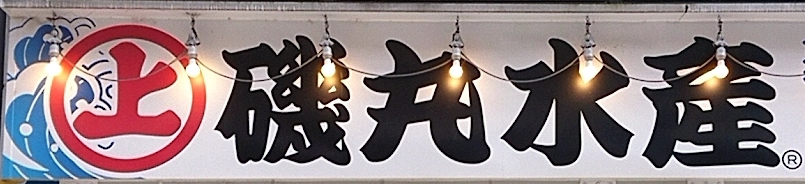
\includegraphics[clip, height=2zh]{isomaru.png}
        \end{minipage} & 
        1.000 & 0.960 & 0.980 & % isomaru
        10 & 10 \\
        (8) & 
        \begin{minipage}{40mm}
          \centering
          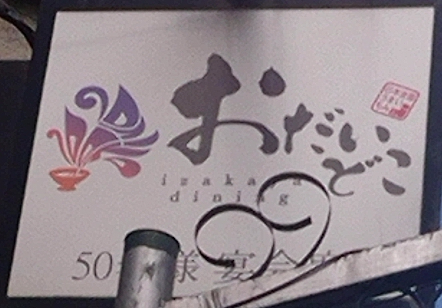
\includegraphics[clip, height=2zh]{odaidoko.png}
        \end{minipage} & 
        1.000 & 1.000 & 1.000 & % odaidoko
        8 & 3 \\
        (9) & 
        \begin{minipage}{40mm}
          \centering
          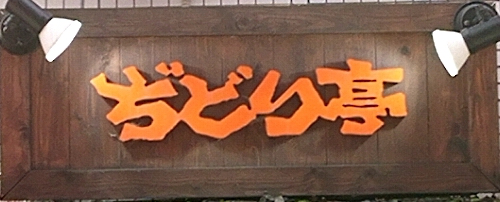
\includegraphics[clip, height=2zh]{jidori.png}
        \end{minipage} & 
        0.955 & 0.840 & 0.894 & % jidori
        10 & 7 \\
        (10) & 
        \begin{minipage}{40mm}
          \centering
          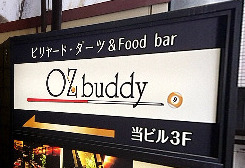
\includegraphics[clip, height=2zh]{ozbuddy.png}
        \end{minipage} & 
        0.962 & 1.000 & 0.980 & % ozbuddy
        10 & 10 \\
        (11) &
        \begin{minipage}{40mm}
          \centering
          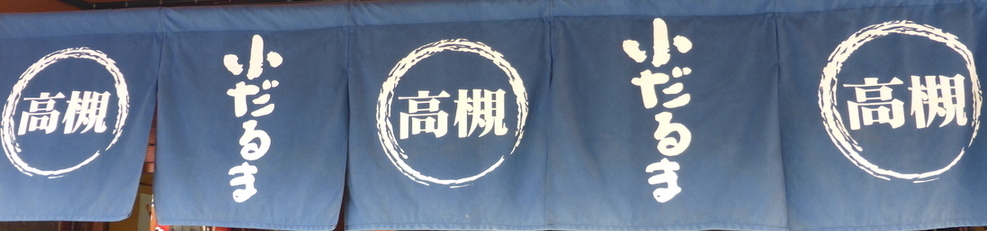
\includegraphics[clip, height=2zh]{kodaruma.png}
        \end{minipage} & 
        1.000 & 0.840 & 0.913 & % kodaruma
        10 & 10 \\
        (12) & 
        \begin{minipage}{40mm}
          \centering
          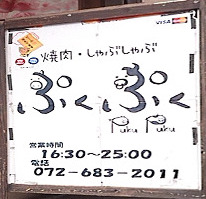
\includegraphics[clip, height=2zh]{pukupuku.png}
        \end{minipage} & 
        1.000 & 0.880 & 0.936 & % pukupuku
        10 & 10 \\
        (13) & 
        \begin{minipage}{40mm}
          \centering
          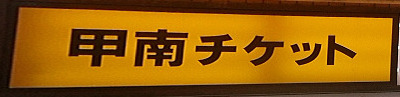
\includegraphics[clip, height=2zh]{konan.png}
        \end{minipage} & 
        1.000 & 1.000 & 1.000 & % konan
        8 & 8 \\
        (14) & 
        \begin{minipage}{40mm}
          \centering
          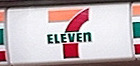
\includegraphics[clip, height=2zh]{seveneleven.png}
        \end{minipage} & 
        1.000 & 0.960 & 0.980 & % seveneleven
        9 & 9 \\
        (15) & 
        \begin{minipage}{40mm}
          \centering
          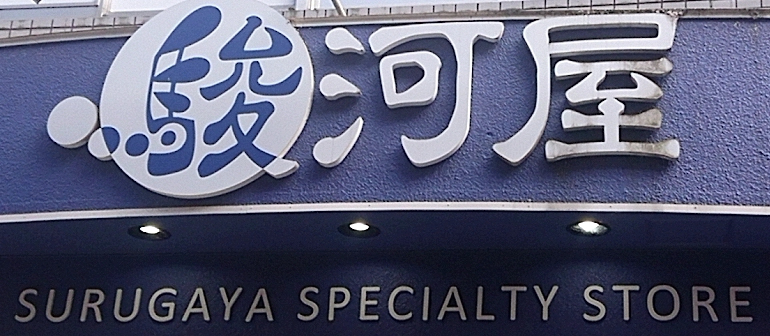
\includegraphics[clip, height=2zh]{surugaya.png}
        \end{minipage} & 
        1.000 & 0.960 & 0.980 & % surugaya
        10 & 10 \\
        \hline
      \end{tabular}
    \end{center}
  \end{table}

  \begin{figure}[tb]
    \centerline{
      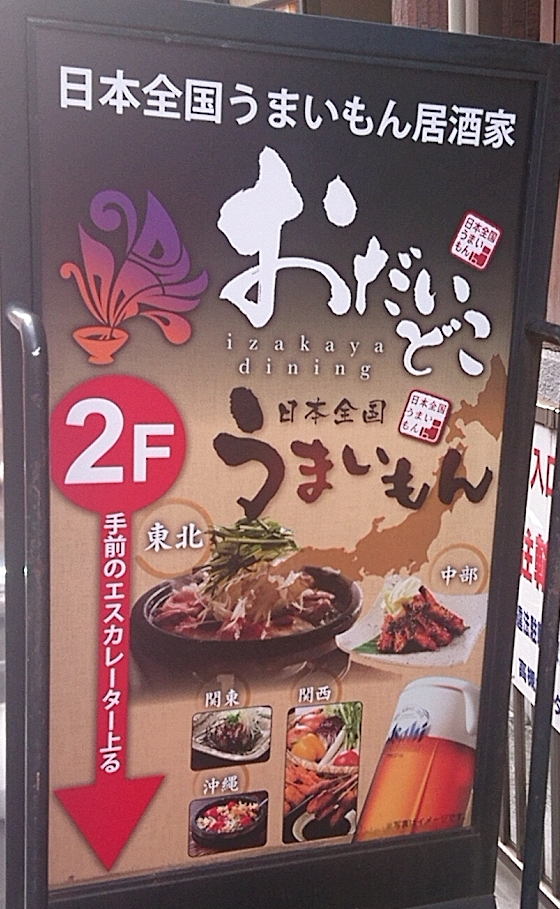
\includegraphics[width=.2\columnwidth, clip]{odaidoko1.png}
      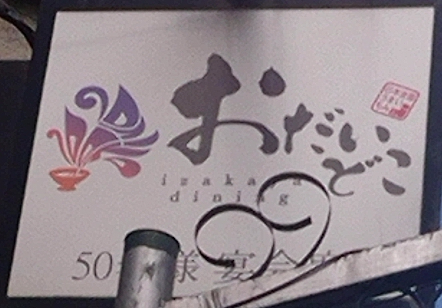
\includegraphics[width=.3\columnwidth, clip]{odaidoko2.png}
      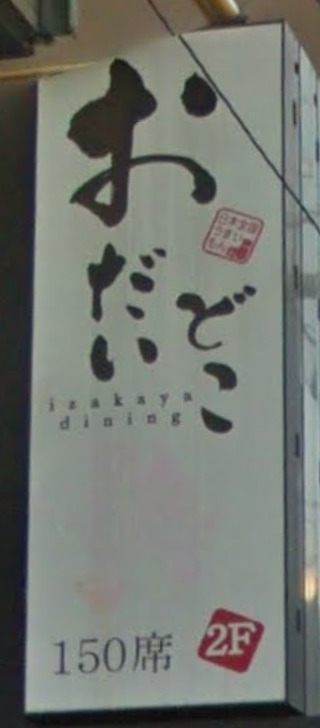
\includegraphics[width=.15\columnwidth, clip]{odaidoko3.png}
      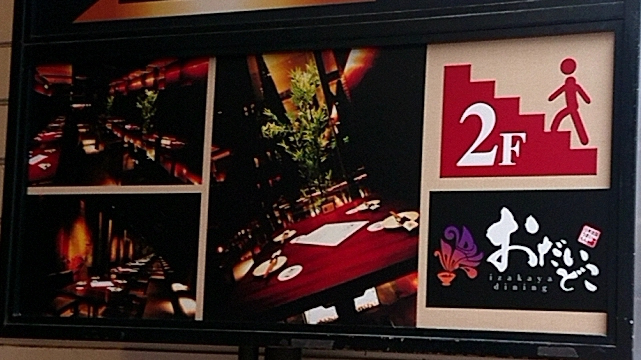
\includegraphics[width=.3\columnwidth, clip]{odaidoko4.png}
    }
    \caption{認識精度が低かった看板の例}
    \label{figure:recog_discussion}
  \end{figure}
